\chapter{Technologies Used}

In this chapter the author will describe the technologies and tools that were used to implement the Thesis Management System. The only requirement of the thesis description was to use platform \emph{Grails} and the requirements of the customer were to use platform \emph{OpenShift} for deployment, \emph{GitHub} for source code hosting and a \emph{GPL} compatible license for licensing.

\section{Groovy}

Groovy is a dynamic object-oriented programming language for the Java platform and therefore ``makes modern programming features available to Java developers with almost-zero learning curve''\cite{groovy-homepage}. Groovy compiles to Java bytecode, so it can be seamlessly integrated with all Java classes and libraries\cite{groovy-homepage}. It has a lot of features that make writing code less verbose and more expressive, like:

\begin{itemize}
    \item Closures -- anonymous functions that can be written on one line without making the readability suffer
    \item Reasonable defaults like public methods, private attributes with default accessors, final classes
    \item Support for Domain Specific Languages, which makes the code one of the most compact among other programming languages
    \item Inferred type system that makes the code more DRY\footnote{Don't Repeat Yourself -- A principle aimed at reducing repetition in programming code}
    \item Null safe operator, Elvis operator
\end{itemize}

As Groovy features a dynamic type system, it makes the code more readable and less verbose, however, as the type checks happens at run time rather than at compile time, the code is more error-prone since a type error is not thrown until the user accesses the affected code\cite{groovy-in-action}.

Groovy is the principal programming language that is used for the implementation of the Thesis Management System since the Grails platform is based on it.

\section{Grails}

``Grails is an Open Source, full stack, web application framework for the Java Virtual Machine. It takes advantage of the Groovy programming language and convention over configuration to provide a productive and stream-lined development experience.''\cite{grails-homepage}. It is a well documented\cite{grails-documentation}, easy to use and easily extensible platform that is designed according to the MVC\footnote{Model--view--controller} paradigm, which divides the application into three components that interact with each other greatly improving the project code's readability and maintainability. The Grails framework uses several well-known Java technologies under the hood, including:

\begin{description}
    \item[Hibernate] -- ORM\footnote{Object-relational mapping -- technique for converting objects into relational database compatible data} framework that is used as layer for data access, Grails wraps its API with Groovy making it much easier to configure and use.
    \item[Spring] -- The most popular application development framework for enterprise Java\cite{springsource-homepage} and a Java EE competitor.
    \item[SiteMesh] -- Web application template framework which follows the decorator design pattern, Grails uses it for GSP\footnote{Groovy Server Pages} views.
\end{description}

To start with Grails, all you need to do is download and install the Grails distribution and then execute command \texttt{grails create-app [name]}, which creates the directory structure and default configuration of your application. You can then write your domain model and, thanks to grails feature called \emph{Scaffolding}, auto-generate the controllers and views for a particular domain class. To start the application, you simply execute \texttt{grails run-app} and the application is launched in development environment on Tomcat 7 servlet container. This experience makes first steps with Grails very easy and fun, the only caveat is that the auto-generated code needs a lot of polishing to improve its readability.

\section{Git and GitHub}

It is nearly impossible to develop a project as big as the Thesis Management System without a version control, therefore you usually need to choose a version control system. There are a lot of options you can choose from including Subversion, Mercurial or CVS. Git is, however, undoubtedly one of the best options as it is the most popular, flexible and scalable VCS\footnote{Version control system} there is. It is designed and developed by Linus Torvalds, a principal software developer of the Linux kernel, and it features very fast branching, decentralized system and a lot of useful commands like \texttt{rebase} or \texttt{squash}\cite{git-homepage}\cite{pro-git}.

GitHub is a source code hosting for projects that use Git as a version control tool. It is free (unless you need a private repository), easy to use web service and with features like forking and code reviewing, it is the most popular code host on the planet\cite{github-features}.

\section{PostgreSQL}

There are many ways you can store data of your application, you can store it in a file or you can use the filesystem hierarchy. These solutions are not, however, scalable enough to handle an amount of work that most applications need and for that reason, more than 30 years ago, Oracle introduced the first relational database management system (RDBMS) that stores data in relational tables. Relational databases developed the best mix of simplicity, performance, scalability and compatibility over the years, and therefore they are the predominant choice in storing data even though they are not suitable for storing of objects of current popular object oriented programming languages like Java. There are, however, many technologies that mitigate these drawbacks like ORM or RowSet. ORM frameworks, for instance, usually provide an API that effectively creates a ``virtual object database''.

To manage data in a relational database, the SQL language was introduced. SQL allows you to select, update, delete or insert data into relational database using an easy declarative syntax. For example, query \texttt{SELECT * FROM thesis} returns all data in the \texttt{thesis} table and query \texttt{DELETE FROM thesis WHERE id = 1} deletes all rows that contain \texttt{1} in column \texttt{id} from table \texttt{thesis}. Modern relational databases support features like triggers, cursors or procedural SQL, which allows you to create the back end of your application entirely in SQL syntax.

One of the most convincing features of relational databases is transaction support. A transaction is a group of operations that have the following properties:

\begin{description}
    \item[Atomicity] -- Either all operations occur, or nothing occurs. This prevents occurring of partial updates to the database.
    \item[Consistency] -- No operations violate integrity constraints.
    \item[Isolation] -- Two concurrent transaction are isolated from changes done by the other.
    \item[Durability] -- When a transaction is finished, all data is saved permanently even if the system, for example, crashes.
\end{description}

There are a lot of relational databases, the most popular are MySQL, SQLite and PostgreSQL, which is the one we chose for the Thesis Management System. This database offers everything most applications require and is easy to configure with a great support.

\section{MongoDB}

MongoDB is a NoSQL database written in C++\cite{mongodb-homepage} that stores data in JSON\footnote{JavaScript Object Notation}-style documents. It features high scalability, master-slave replication, load balancing, file storage and, as well as regular relational databases, it supports indexes on attributes. 

In the past 5 years, NoSQL databases have been getting more popular with MongoDB on top\cite{db-ranking}. This happens mostly because relational databases are hard to scale and mapping objects on JSON objects is much easier than on tables, even if you use a really good ORM framework. Another reason is that objects in dynamic languages tend to change number of attributes at runtime, with MongoDB, all attributes get stored because MongoDB offers dynamic schemas.

MongoDB, as opposed to relational databases, does not store data in tables. Instead of tables, MongoDB stores data in collections of documents, so a table in a relational database is equivalent to a collection in MongoDB and a row in a table is equivalent to a document. In practice, if you develop an application in an OO\footnote{Object Oriented} programing language, with a relational database, a table usually represents a class (or type) and a table row represents an instance of a class, but if you use MongoDB, a collection represents a class and a document represents an instance.

CRUD\footnote{Create, Read, Update, Delete} operations in MongoDB are much more user friendly for people that are familiar with OO programing languages. Read operations are done via a query with the following syntax:

\begin{verbatim}
db.collection.find( <query>, <projection> )
\end{verbatim}

Where the \texttt{<query>} argument corresponds to the \texttt{WHERE} statement of an SQL \texttt{SELECT} query and \texttt{<projection>} argument corresponds to the set of arguments following an SQL \texttt{SELECT} query. Write operations follows the same syntax but instead of \texttt{find} method, you use either \texttt{insert}, \texttt{update} or \texttt{remove} method.

There are some drawbacks a newcomer from RDBMS must consider, though. If you choose MongoDB for a project, you must manage transactions in your application logic, because MongoDB does not support them. And write operations are atomic only on the level of a single document. You cannot count on integrity constraints either, because MongoDB does not have any apart from the very basic ones. All these drawbacks can be mitigated by a good framework but it is recommended to consider the choice of a database storage carefully.

\section{OpenShift}

OpenShift is Red Hat's Cloud Computing \emph{Platform as a Service} offering\cite{openshift-homepage}. Platform as a Service (PaaS) offerings facilitate the deployment of web-based applications without the cost and complexity of buying servers and setting them up\cite{guardian-google-paas}. In short, this means that you can set up your production environment with all software needed (database, application server) in a matter of minutes and you can deploy your application by one command-line command.

\begin{figure}[htbp]
    \centering
        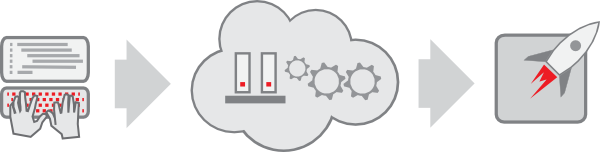
\includegraphics[scale=0.5]{./images/overview-paas.png}
    \caption{Platform as a Service overview}
    \label{fig:overview-paas}
\end{figure}

Red Hat is an open-source company, i.e. every project developed by Red Hat is open-source -- and so is OpenShift. OpenShift is build on RHEL\footnote{Red Hat Enterprise Linux}, which is a stable Linux distribution with long-term support, it is written in Ruby programming language and it runs your applications on Amazon EC2\footnote{Amazon Elastic Compute Cloud -- cloud computing platform that allows users to rent virtual computers}.

Creating your first application on OpenShift is very straightforward. First, you choose a type of application, which is called a cartridge in OpenShift terminology. You can choose from a variety of cartridges including, for example, JBoss Application Server, Tomcat 7, Ruby on Rails and Django, or you can choose the Do It Yourself cartridge and set up the whole environment yourself. Once you have done that, you choose a public URL, a source code repository, gears and scaling. A gear is a container with limited resources that runs your application, i.e. virtual server. By default, you can only choose the default small gear. If you pay a monthly fee, you can choose medium or large gear with more resources at your disposal. Scaling allows your application to be load-balanced, i.e. if your applications' traffic increases, OpenShift will allocate more gears. When you have your application created, you can do some basic configuration through the web interface or you can add another cartridge to your application, e.g. a database or Cron. If you need to connect to the server where your application runs, you can open a Secure Shell session (supposing you've set up your public RSA key). This overall flexibility decreases time spent managing software and hardware, and it makes it easy to deploy your application without any fuss, so at least from that point of view, it makes sense to use OpenShift even if you have no choice but to use the Do It Yourself cartridge.

If setting up a new OpenShift application is simple, deploying one is even more simple. You just push the application's source code to either the repository you specified or the repository that was created for you. You might need to set some properties in your application (e.g. database credentials), though. Fortunately, OpenShift exports all needed properties as environment variables so that you could access them via the API of your programming language and use them wherever necessary. If you need to inject or modify some environment variables at some point (e.g. before or after build), you can use action hooks. These lifecycle hooks allows you to execute any kind of shell script at a certain point in time, for example, you might want to append a property to the \texttt{JAVA\_OPTS} environment variable just before the build of your application. To do that, you put the following script in \texttt{\$\{project.dir\}/.openshift/action\_hooks/pre\_build}:

\begin{verbatim}
#!/bin/bash
export JAVA_OPTS="$JAVA_OPTS -DsomeProperty=true"
\end{verbatim}

The script above gets executed directly, so you can use PHP, Python, Ruby or any other interpreted programing language.

\section{Others}

There are a lot of other technologies used for the implementation of the Thesis Management System, to keep it short, the author will describe them just briefly.

\begin{description}
    \item[Spring Security] -- A Spring framework that provides authentication and authorization for Java.
    \item[Searchable] -- Grails plugin that adds search functionality based on Compass and Apache Lucene\cite{searchable-documentation}.
    \item[JQuery] -- The most popular JavaScript framework.
    \item[LESS] -- CSS preprocessor featuring e.g. variables, mixins, operators and nesting.
    \item[Twitter Bootstrap] -- CSS framework and the most popular project on GitHub.
\end{description}

